% 原文 pp.154–161（印刷 pp.1272–1279）
% 原文 §11.5（续）：三孔球面上的路径积分、配分函数的拼装与模空间上的相交理论

% ===== 原文 p.154 =====
% （本页首句承接 p.153 末段：(11.32) 中的常数 $\alpha$ 乘在 $\Sigma$ 的 Euler 示性数上。）
……它最终会被调整，以确保配分函数的整体归一化及其对亏格 $g$ 的依赖，与用其他方法（例如在特殊情形下作显式计算）所得的结果一致。

要为拼装出任意 Riemann 面准备好「零件」，我们还必须考虑特殊曲面 $\mathcal{P}$ 上的场论；$\mathcal{P}$ 是一张挖去三个圆盘的球面（即三孔球面（trinion），或称「裤子」（pair of pants）：见图 1（原文 Figure 1））。

\begin{figure}[htbp]
  \centering
  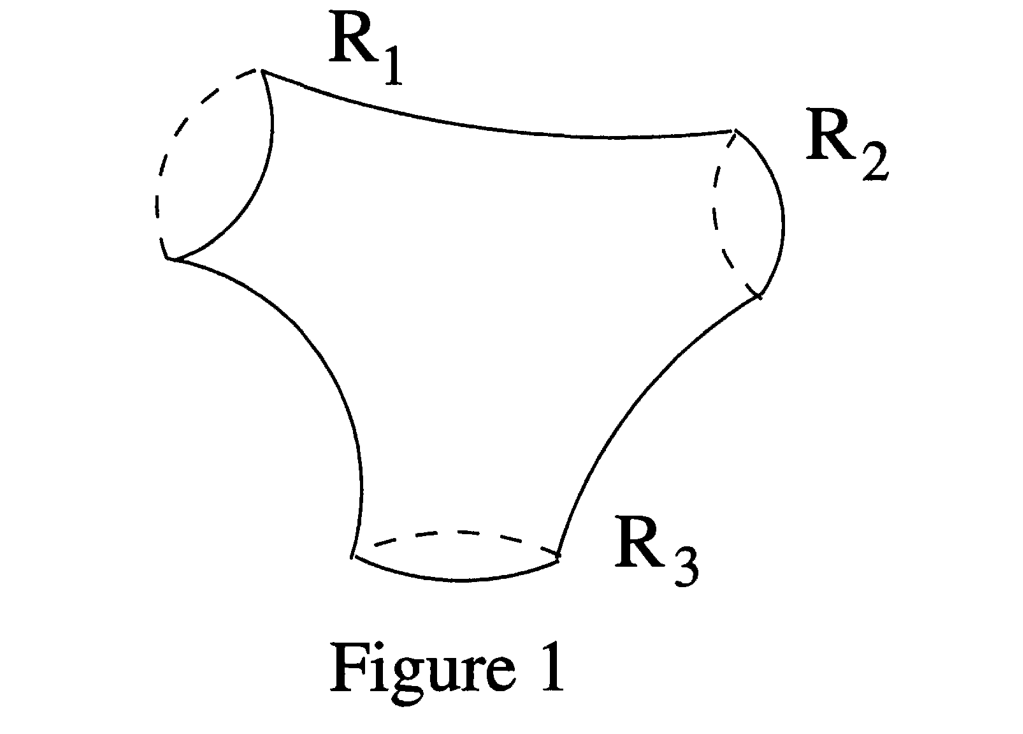
\includegraphics[width=0.52\textwidth]{figs/fig_p154_1.png}
  \caption{三孔球面（trinion，亦称「裤子」）：由球面挖去三个圆盘得到，三条边界分支分别标记为 $R_1$、$R_2$、$R_3$（虚线表示被挖去的圆盘的边沿）。（原文 Figure 1，p.154）}
  \label{fig:p154-1}
\end{figure}

我们设想在 $\mathcal{P}$ 上作路径积分，并在各边界分支上插入态 $\Psi_{R_i}$（$i=1,2,3$）。这个路径积分是
\begin{equation}
  \tag{11.33}
  \label{eq:11-33}
  W_{R_1R_2R_3}=\int \mathcal{D}A\,\exp(-\mathcal{L})\prod_{i=1}^{3}\Psi_{R_i}(A|_{C_i}),
\end{equation}

% ===== 原文 p.155 =====
其中 $A$ 取遍 $\mathcal{P}$ 上丛的联络空间。对任意的 $R_i$ 算出这个路径积分之后，把各部分拼装起来就相当直接了。

第一步是证明：除非诸 $R_i$ 全都相同，路径积分 $W_{R_1R_2R_3}$ 为零。我们在 $\mathcal{P}$ 中的某点 $p$ 处插入与可观测量 $Q_S^{(0)}(p)$ 相应的算符 $\widehat{Q_S^{(0)}}(p)$。我们假定 $p$ 靠近某个以表示 $R$ 标记的边界分支（$R$ 是诸 $R_i$ 之一）。于是可以认为算符 $\widehat{Q_S^{(0)}}(p)$ 作用在态 $\Psi_R$ 上。（这一点已在图 2（原文 Figure 2）中示意：那里算符插入被标记为 $S(F)$，并被看作作用在态 $\Psi_{R_1}$ 上。）利用 (11.30) 及其对高阶 Casimir 算符的推广，我们看到态 $\Psi_R$ 是 $\widehat{Q_S^{(0)}}(p)$ 的本征态，本征值为某个 $C(S,R)$：
\begin{equation}
  \tag{11.34}
  \label{eq:11-34}
  \widehat{Q_S^{(0)}}(p)\Psi_R=C(S,R)\Psi_R .
\end{equation}

\begin{figure}[htbp]
  \centering
  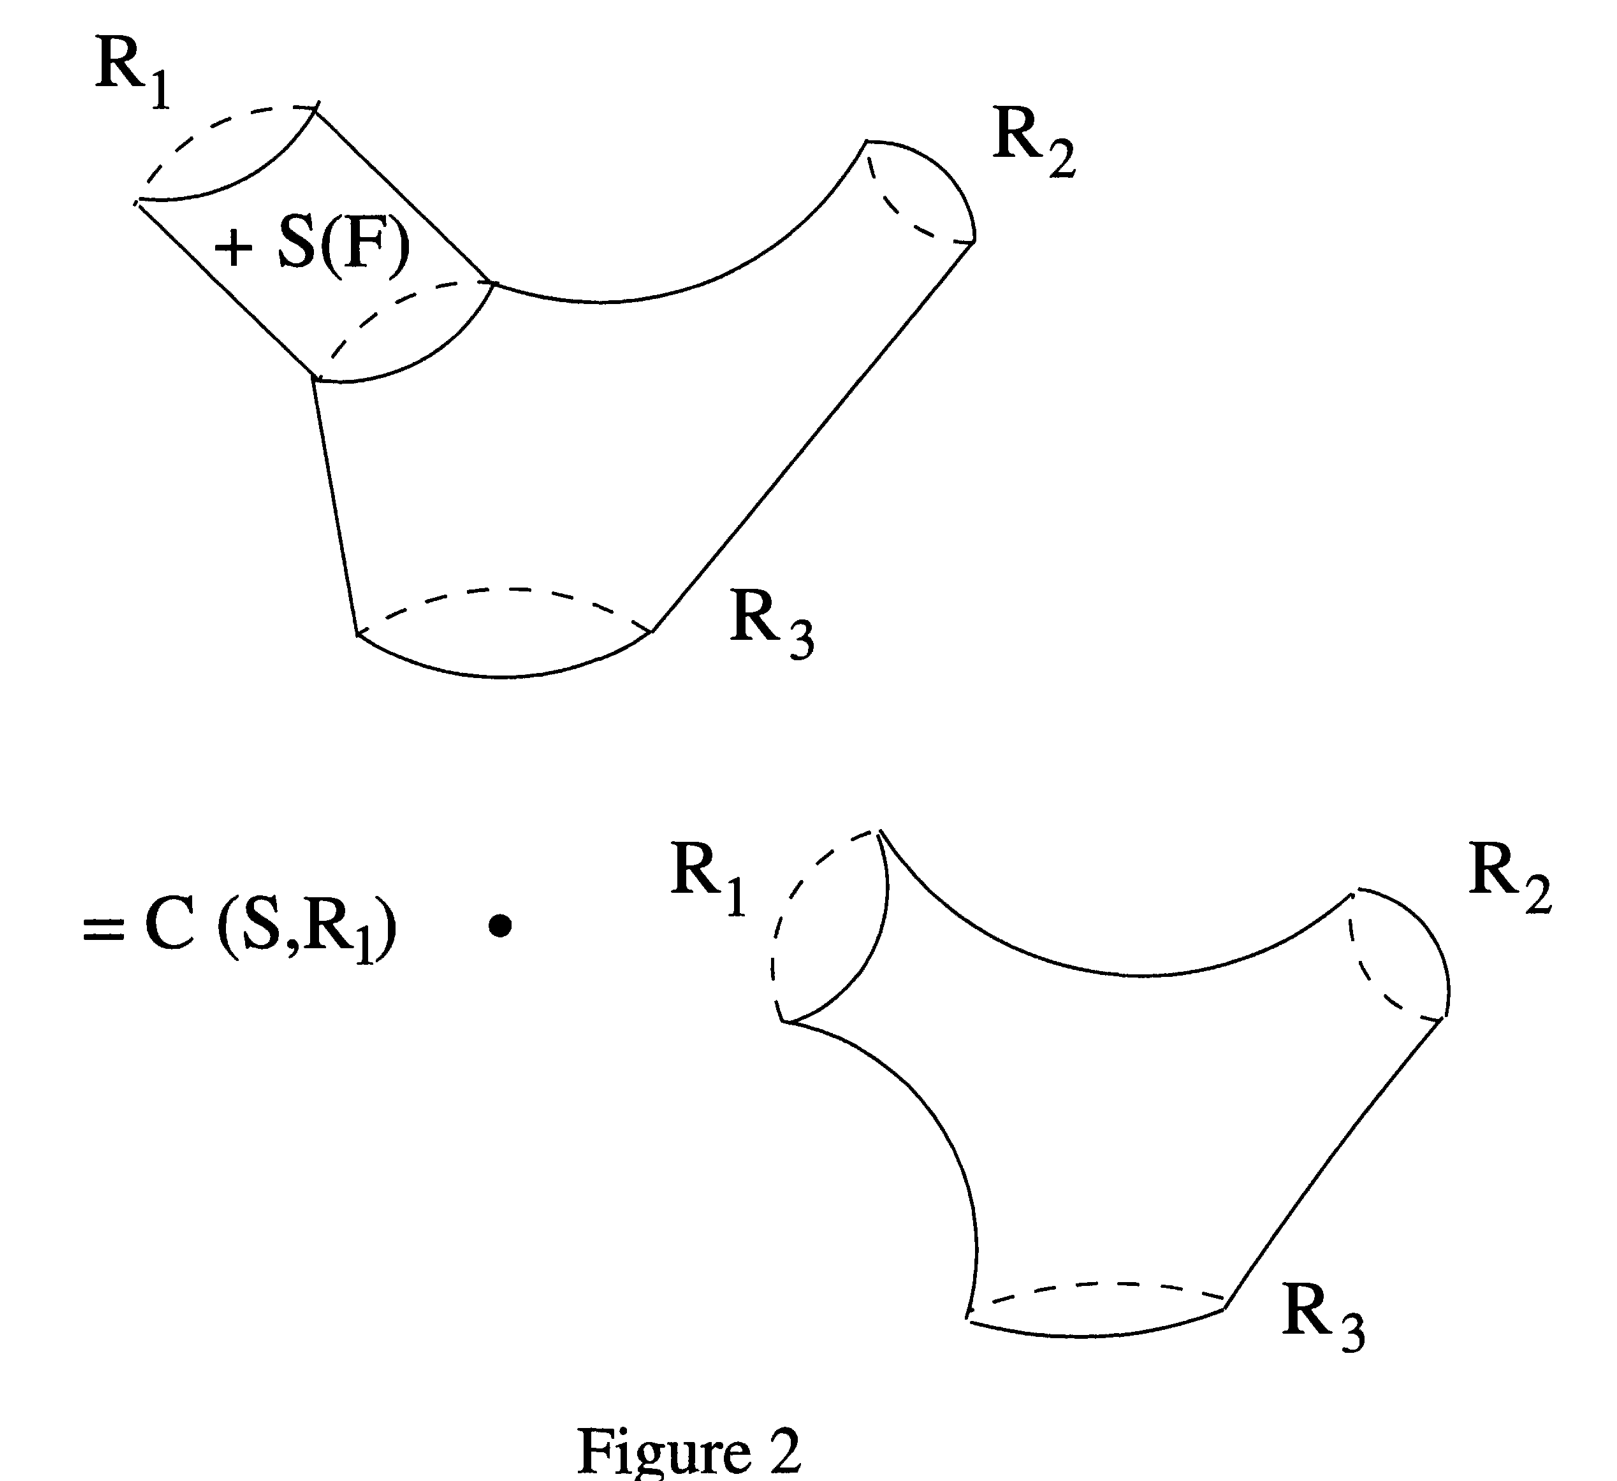
\includegraphics[width=0.60\textwidth]{figs/fig_p154_2.png}
  \caption{在 $R_1$ 所标记的边界分支附近插入算符（图中标为 $+S(F)$）的三孔球面路径积分，等于常数 $C(S,R_1)$ 乘以未插入算符的三孔球面路径积分（图中圆点表示乘法）。（原文 Figure 2，p.154）}
  \label{fig:p154-2}
\end{figure}

这里，若 $S$ 是 $\mathfrak{g}$ 上次数为 $l$ 的不变多项式，则 $C(S,R)$ 就是表示 $R$ 相应的 $l$ 阶 Casimir。（例如，若 $S$ 是规范不变函数 $S(\phi)=\mathrm{Tr}(\phi^{l})$，其中 $\mathrm{Tr}$ 取在伴随表示上，则量子化后 $S$ 成为 $\mathrm{Tr}(\delta/\delta A)^{l}$ 的某个倍数。$\Psi_R$ 是此算符的本征态，本征值为 $C(S,R)$ 的某个倍数。）由于 $R$ 可以取 $R_1$、$R_2$ 或 $R_3$ 中的任何一个，我们发现这个单点函数等于 $C(S,R_j)W_{R_1R_2R_3}$（$j=1,2,3$），其中 $W_{R_1R_2R_3}$ 如上定义。这一论断成立的理由如下：由于该场论在保面积微分同胚（area preserving diffeomorphism）下不变，我们可以把算符插入放在我们所选定的任何一条边界分支附近，因此该算符可以被看作作用在任何一个外态上。由此可见，对每个 $j$，Casimir 值 $C(S,R_j)$ 全都相等；又因这对所有不变多项式 $S$ 都成立，故只要 $W(R_1,R_2,R_3)\neq0$，就必须有 $R_1=R_2=R_3$。

% [Tutor Note: 由 (11.30) 到 (11.34) 的关键是把 $\phi^{a}$ 换成泛函导数 $\delta/\delta A^{a}$（见 p.153 的 (11.29)），于是 $S(\phi)=\mathrm{Tr}(\phi^{l})$ 量子化后确实是一个 $l$ 阶线性微分算符 $\mathrm{Tr}(\delta/\delta A)^{l}$。诸 $\delta/\delta A^{a}(x)$ 彼此对易，故此处无算符排序歧义——但也正因如此，$\Psi_R$ 是真正的本征态而不仅是广义本征态。易错点：式中的 $\mathrm{Tr}$ 必须取在伴随表示上（原文如此）；若误取基本表示，$C(S,R)$ 就不再是 $R$ 的 Casimir 而是别的缩并，于是「三个边界分支的 Casimir 相等 $\Rightarrow R_1=R_2=R_3$」这一步失效。]

于是问题归结为计算 $\mathcal{P}$ 的配分函数，其边界条件由三条边界分支上同一个外态 $\Psi_R$ 决定。把这个配分函数在零面积极限下的值记为 $w_R$。那么面积依赖关系是：若面积为 $a$，则得到
\begin{equation}
  \tag{11.35}
  \label{eq:11-35}
  Z_R=w_R\exp\left(-\tilde{c}_2(R)\frac{ae^{2}}{2}\right),
\end{equation}
这里我们现用 $Z_R$ 表示 $W_{R,R,R}$。面积依赖关系必定如此，理由是我们可以在任一边界分支上粘上一个给定面积的圆柱来增大三孔球面的面积；这会把 $Z_R$ 乘以在把 $\Psi_R$ 沿给定面积传播时出现的因子 (11.31)。

% [Tutor Note: (11.35) 中出现的是 $\tilde{c}_2$ 而非 $c_2$，这不是笔误，而是 (11.32) 重整化效应的体现：$\tilde{c}_2(R)=c_2(R)+\beta$，常数移位 $\beta$ 在 (11.35) 里给出一个与 $R$ 无关的因子 $e^{-e^{2}a\beta/2}$，可并入 $w_R$；p.160 的 $c_2(R_n)=(n^{2}-1)/2\to\tilde{c}_2(R_n)=n^{2}/2$ 正是 $\beta=1/2$。另外要看清「面积依赖只能是这一个指数」的真正依据：圆柱传播子 (11.31) 只含 $e^{-e^{2}a\,c_2/2}$ 一个因子，故 $\ln Z_R$ 对 $a$ 必须是线性的，这就排除了 $\ln Z_R$ 中出现 $a^{2}$ 等高次项的可能——等价地说，二维 Yang--Mills 是超可重整化理论，作用量中可用的一次项只有 $\int\mathrm{tr}\,F^{2}$ 与 $\int R$（后者见 (11.32)）。]

现在我们来考虑亏格为 $g$、无边界 Riemann 面的配分函数的计算问题。这样的曲面可以由 $2g-2$ 个 $\mathcal{P}$ 的副本 $\mathcal{P}_j$ 沿 $3g-3$ 条边界圆 $C_\gamma$ 粘合而成。我们可以按场在边界圆 $C_\gamma$ 上的限制值来分解配分函数的路径积分。若 $A'$ 表示诸 $\mathcal{P}_j$ 的边界圆 $\coprod_\gamma C_\gamma$ 上一个联络的取值，而 $\mathcal{A}_{A'}=\{A\in\mathcal{A}:\ A|_{\coprod_\gamma C_\gamma}=A'\}$ 是

% ===== 原文 p.156 =====
所有限制到给定边界值 $A'$ 的联络之集合，则我们有\footnote[3]{见本讲末尾参考文献中所列 Witten 第一篇论文的 §4.5。}
\begin{equation}
  \tag{11.36}
  \label{eq:11-36}
  \int_{\mathcal{A}}\mathcal{D}A\,e^{-\mathcal{L}}=\int \mathcal{D}A'\int_{\mathcal{A}_{A'}}\mathcal{D}A\,e^{-\mathcal{L}} .
\end{equation}
这里，右端的 $DA$ 是对那些在诸 $C_\gamma$ 上限制为 $A'$ 的 $A$ 所作的积分。一旦固定了诸 $C_\gamma$ 上的联络 $A'$，空间 $\mathcal{A}_{A'}$ 就是 $2g-2$ 个 $\mathcal{P}$ 上联络空间（带指定的边界值）的乘积。$\mathcal{P}$ 在给定联络边界值与面积 $a$ 下的配分函数为
\begin{equation}
  \tag{11.37}
  \label{eq:11-37}
  Z(\mathcal{P},A|_{\partial\mathcal{P}})=\sum_{R}w_R\prod_{\gamma=1}^{3}\Psi_R(A|_{C_\gamma})\exp\left(-\frac{e^{2}a\tilde{c}_2(R)}{2}\right).
\end{equation}
（鉴于诸 $\Psi_R$ 的正交性，这与 (11.35) 等价。）要还原亏格 $g$ 的闭 Riemann 面 $\Sigma$ 的配分函数，我们把 $2g-2$ 个 $Z(\mathcal{P})$ 相乘并对边界值 $A'$ 积分。利用与诸态 $\Psi_R$ 相对应的群特征标的正交关系，我们得知：只有当 $2g-2$ 个三孔球面中每一个上面的诸 $R$ 全都相同时，才出现非零贡献。对 $R$ 求和给出
\begin{equation}
  \tag{11.38}
  \label{eq:11-38}
  Z(\Sigma)=\sum_{R}w_R^{2g-2}\exp\left(-\frac{e^{2}a\tilde{c}_2(R)}{2}\right).
\end{equation}
（当然，此时 $a$ 是整个曲面的面积。）

现在我们来解释如何计算 $w_R$。我们注意到，面积为 $a$、边界上有外态 $\Psi_R$ 的圆盘 $D$ 的配分函数是
\begin{equation}
  \tag{11.39}
  \label{eq:11-39}
  Z_R(D)=v_R\exp\left(-\frac{e^{2}a\tilde{c}_2(R)}{2}\right),
\end{equation}
其中 $v_R$ 为某个常数。面积依赖关系由通常的因子给出，因为同样地，我们可以通过给边界粘上一个给定面积的圆柱来改变面积。

边界条件由两个边界分支上的波函数 $\Psi_R$（相应地 $\Psi_{R'}$）所决定的圆柱，其配分函数当 $R\neq R'$ 时等于 $0$，因为 $\Psi_R$ 是 Hamilton 量 $H$ 的本征函数。（见

\begin{figure}[htbp]
  \centering
  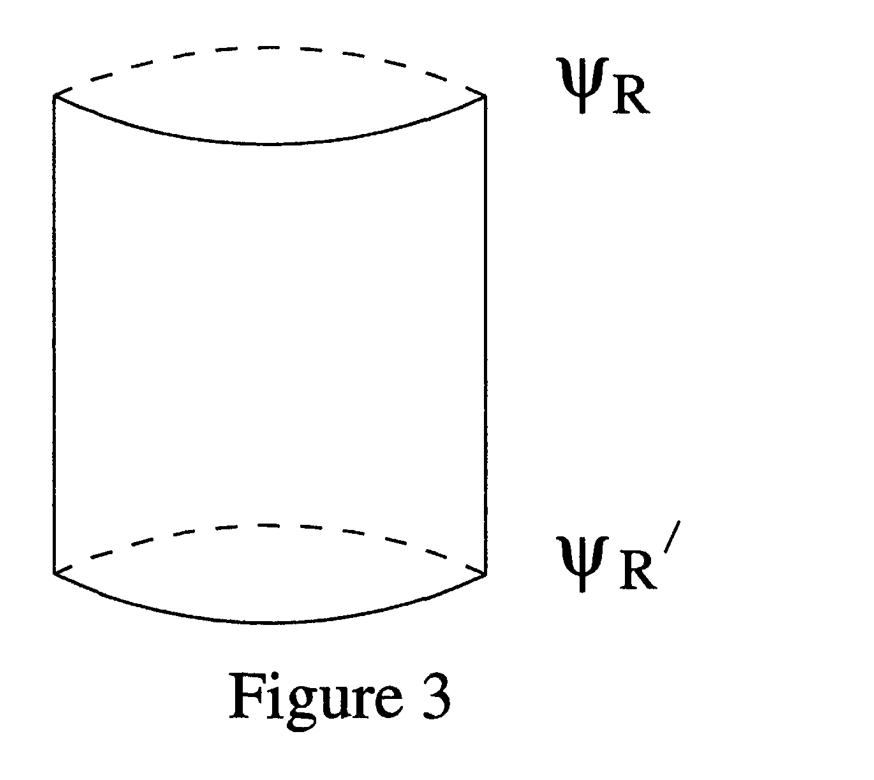
\includegraphics[width=0.40\textwidth]{figs/fig_p156_1.png}
  \caption{圆柱 $S^{1}\times I$：两个边界分支上分别带有外态 $\Psi_R$（上）与 $\Psi_{R'}$（下）。当 $R\neq R'$ 时其配分函数为零。（原文 Figure 3，p.156）}
  \label{fig:p156-1}
\end{figure}

% ===== 原文 p.157 =====
图 3。）面积为 $a$、两个边界分支上都有外态 $\Psi_R$ 的圆柱 $S^{1}\times I$ 的配分函数为
\begin{equation}
  \tag{11.40}
  \label{eq:11-40}
  Z_R(S^{1}\times I)=1\cdot\exp\left(-\frac{e^{2}a\tilde{c}_2(R)}{2}\right)
\end{equation}
（因为诸 $\Psi_R$ 是 Hamilton 量 $H$ 的本征态，而圆柱上的路径积分计算的是 $e^{-HT}$；注意，由于其 Hamilton 量解释，这个公式与前面几个公式不同，不含任何未知的乘性常数）。我们可以像图 4（原文 Figure 4）那样分解圆柱：这给出「两个边界分支上都有外态 $\Psi_R$ 的圆柱」的配分函数，它等于「所有边界分支上都有外态 $\Psi_R$ 的 $\mathcal{P}$」的配分函数与 $D$ 的配分函数之积，于是
\begin{equation}
  \tag{11.41}
  \label{eq:11-41}
  w_R\cdot v_R=1 .
\end{equation}
要确定 $v_R$，只需考虑面积非常小的圆盘 $D$。若把 $D$ 边界上一个联络的和乐（holonomy）固定为取值 $U\in G$，则圆盘的配分函数（限制到 $D$ 上边界和乐为 $U$ 的联络）为（由 (11.39) 并利用特征标的正交性）
\begin{equation}
  \tag{11.42}
  \label{eq:11-42}
  Z(U)=\sum_{R}v_R\chi_R(U)\exp\left(-\frac{e^{2}a\tilde{c}_2(R)}{2}\right)
\end{equation}
（其中 $\chi_R$ 如上所述，表示 $R$ 的特征标）。如果我们改用路径积分来计算配分函数，则把作用量写成
\begin{equation}
  \tag{11.43}
  \label{eq:11-43}
  I(U)=\frac{1}{4e^{2}}\int_D d\mu\,\mathrm{Tr}(|F|^{2}),
\end{equation}
以及
\begin{equation}
  \tag{11.44}
  \label{eq:11-44}
  Z(U)=\int_{\mathrm{Hol}(A)=U}\mathcal{D}A\,\exp\left(-\frac{1}{4e^{2}}\int_D d\mu\,\mathrm{Tr}(|F|^{2})\right),
\end{equation}
（其中我们限制到边界和乐为 $U$ 的联络）。这个积分给出 $U$ 的一个正函数，因为被积函数是正的。当 $e^{2}$（等价地，面积）趋于零时，$Z(U)$ 的支集收敛到 $U=1$，因为任何和乐固定为 $U\neq1$ 的构型，其作用量当 $e\to0$ 时都发散。因此当 $e\to0$ 时，该积分收敛到支撑在 $U=1$ 处的 delta 函数。这给出
\begin{equation}
  \tag{11.45}
  \label{eq:11-45}
  Z(U)=\exp(\alpha)\cdot\delta(U-1),
\end{equation}
这里 $\alpha$ 是一个迄今未知的常数。我们将会看到，它本质上就是 (11.32) 中乘在 Riemann 面 Euler 示性数上的那个常数。把 (11.44) 与 (11.41) 的 $e\to0$ 极限作比较，我们看到
\begin{equation}
  \tag{11.46}
  \label{eq:11-46}
  \exp(\alpha)\delta(U-1)=\sum_{R}v_R\chi_R(U).
\end{equation}
若把此式两端乘以 $\chi_{R'}(U)$ 并对 $U$ 积分，利用群特征标的正交关系，我们得到
\begin{equation}
  \tag{11.47}
  \label{eq:11-47}
  v_R=\exp(\alpha)\dim R,
\end{equation}
从而
\begin{equation}
  \tag{11.48}
  \label{eq:11-48}
  w_R=\frac{\exp(-\alpha)}{\dim R}.
\end{equation}

% [Tutor Note: 原文「Comparing (11.44) to the $e\to0$ limit of (11.41)」中的 (11.41) 应为 (11.42)。(11.41) 是纯数等式 $w_Rv_R=1$，与 $U$ 无关，无法与 (11.44) 相比较；只有 (11.42) 在 $e\to0$（指数因子 $\to1$）时化为 $\sum_R v_R\chi_R(U)$，才与 (11.45) 的 $\exp(\alpha)\delta(U-1)$ 相等，从而得到 (11.46)。此处按原文照译并加注。]

% [Tutor Note: (11.46)$\to$(11.47) 用的是 Peter--Weyl 关系 $\delta(U-1)=\sum_R(\dim R)\chi_R(U)$ 与 $\int dU\,\chi_R(U)\chi_{R'}(U)=\delta_{RR'}$（Haar 测度取归一化 $\int dU=1$）。由此 $v_R=e^{\alpha}\dim R$，再配合 (11.41) 得 $w_R=e^{-\alpha}/\dim R$。易错点：若把 $\chi_R$ 换成归一化特征标 $\hat\chi_R=\chi_R/\dim R$（作者在 (11.53)、(11.55) 中正是用 $\hat\chi_R$），则 delta 函数的展开须写成 $\delta(U-1)=\sum_R(\dim R)^{2}\hat\chi_R(U)$，否则 (11.47)、(11.48) 中的 $\dim R$ 因子会整体错位。]

% ===== 原文 p.158 =====
\begin{figure}[htbp]
  \centering
  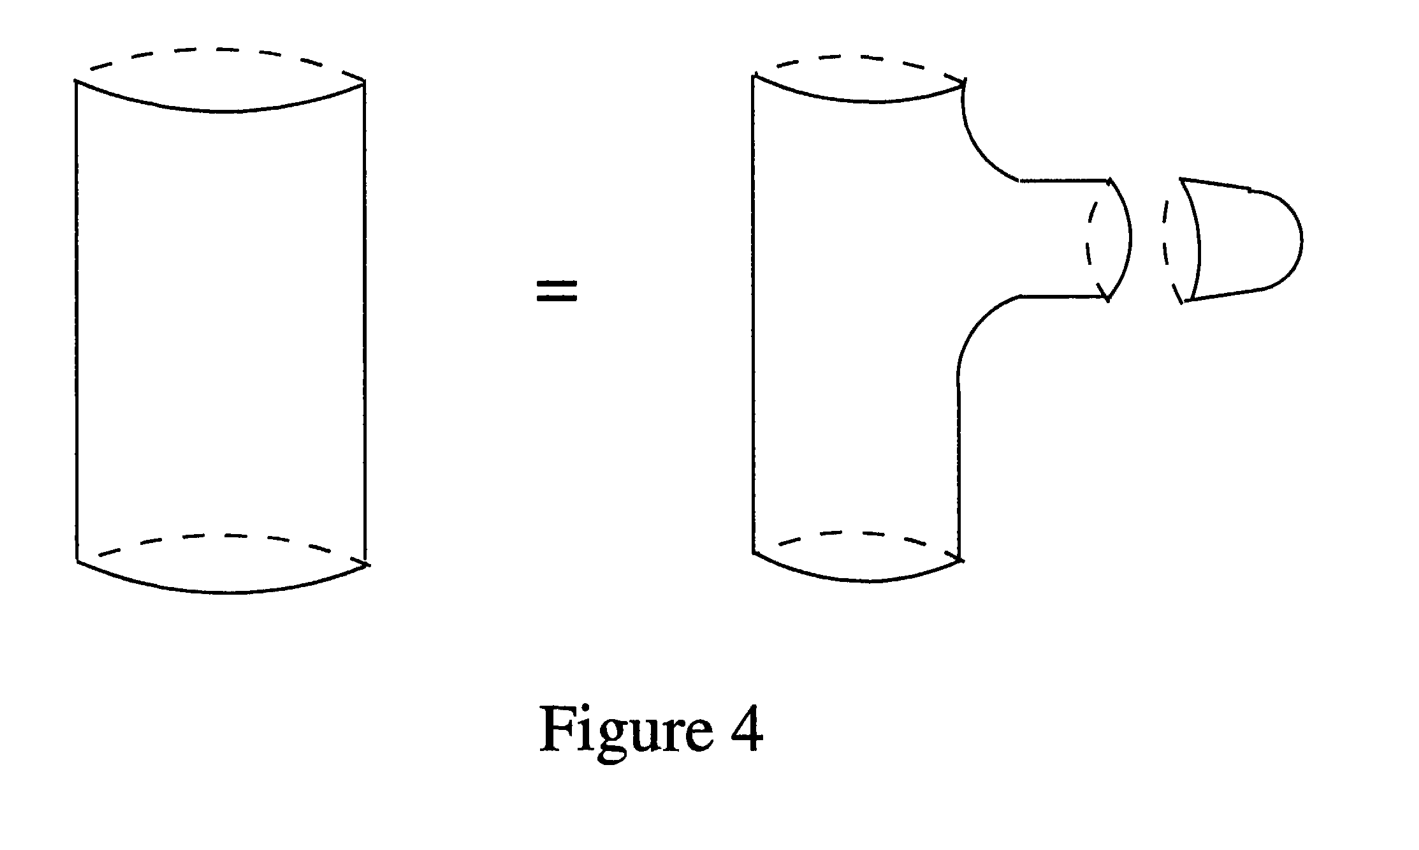
\includegraphics[width=0.62\textwidth]{figs/fig_p158_1.png}
  \caption{圆柱的分解：圆柱 $=$ 三孔球面 $\mathcal{P}$（左）与圆盘 $D$（右）沿一条边界圆粘合；等式表示两边配分函数相乘。（原文 Figure 4，p.158）}
  \label{fig:p158-1}
\end{figure}

于是配分函数为
\begin{align}
  \tag{11.49}
  \label{eq:11-49}
  Z(\Sigma^{g},e^{2}a)&=\sum_{R}w_R^{2g-2}\exp\left(-\frac{\tilde{c}_2(R)e^{2}a}{2}\right)\\
  \tag{11.50}
  \label{eq:11-50}
  &=\sum_{R}\frac{e^{-\alpha(2g-2)}\exp\left(-\tilde{c}_2(R)\varepsilon/2\right)}{(\dim R)^{2g-2}},
\end{align}
其中我们引入了 $\varepsilon=e^{2}a$。

我们刚刚完成的计算给出的是对应于所有可能拓扑类型的 $G$-丛的配分函数之和（回忆一下：若 $G$ 不是单连通的，则 $\Sigma$ 上一般会有若干不同拓扑类型的丛）。要研究某一个特定拓扑类型的贡献，我们取 $G$ 为单连通，并选取一个元素 $\zeta\in Z(G)$（$G$ 的中心）。在 $\Sigma$ 上选一点 $p$，我们限制到 $\Sigma-\{p\}$ 上绕 $p$ 的和乐等于 $\zeta$ 的那些联络。这样的联络会下降为结构群是 $G/Z(G)$ 的商丛上的光滑联络，其拓扑由 $\zeta$ 决定。我们即将大量使用「$G$-丛上具有所述类型奇性的联络」与「$G/Z(G)$-丛上的光滑联络」之间的这一关系。

要把计算推广到带这类奇性的 $G$-丛，我们需要算出包含奇点 $p$（绕 $p$ 的规定单值性（monodromy）为 $\zeta$）的小圆盘 $D$ 上的配分函数，把它表示为圆盘边界上绕行和乐 $U$ 的函数。然后，把 $D$ 粘进任意 Riemann 面，我们就得到该 Riemann 面在包含奇点 $p$ 时的配分函数。在 $e\to0$ 极限下，$D$ 上的配分函数（通过量子化）由
\begin{equation}
  \tag{11.51}
  \label{eq:11-51}
  \sum_{R}u_R\chi_R(U)
\end{equation}
给出，其中 $u_R$ 未知；而（通过路径积分）由
\begin{equation}
  \tag{11.52}
  \label{eq:11-52}
  \exp(\alpha)\delta(U-\zeta)
\end{equation}
给出。后一论断的依据是：若绕 $p$ 的单值性是 $\zeta$，但绕圆盘边界的单值性为 $U\neq\zeta$，则路径积分中的最小作用量在 $e\to0$ 时发散，路径积分将为零；因此该路径积分在 $e\to0$（或小面积）极限下是 $\delta(U-\zeta)$ 的正倍数。

% ===== 原文 p.159 =====
若我们乘以 $\chi_{R'}(U)$ 并对 $U$ 积分，则由特征标的正交性可得
\begin{equation}
  \tag{11.53}
  \label{eq:11-53}
  u_R=\exp(\alpha)\chi_R(\zeta)=\exp(\alpha)(\dim R)\hat{\chi}_R(\zeta),
\end{equation}
其中 $\hat{\chi}_R(\zeta)\in U(1)$ 是表示 $R$ 的归一化特征标在 $\zeta$ 处的取值。现在，若把 $2g-1$ 个 $\mathcal{P}$ 的副本与一个圆盘 $D$ 粘合起来，构成亏格为 $g$ 的闭 Riemann 面，则对配分函数我们得到
\begin{align}
  \tag{11.54}
  \label{eq:11-54}
  Z(\varepsilon,g,\zeta)&=\sum_{R}w_R^{2g-1}e^{-\tilde{c}_2(R)e^{2}a/2}u_R\\
  \tag{11.55}
  \label{eq:11-55}
  &=\sum_{R}\frac{e^{-\alpha(2g-2)}e^{-\varepsilon\tilde{c}_2(R)/2}}{(\dim R)^{2g-2}}\hat{\chi}_R(\zeta).
\end{align}
这是亏格 $g$、带一个穿刺点（puncture）、且绕该穿刺点的和乐为 $\zeta$ 的 Riemann 面上 $G$-联络的配分函数。而我们想要的是相应的 $G/Z(G)$-丛上光滑 $G/Z(G)$-联络的配分函数，该丛的特征类由 $\zeta$ 决定。

% [Tutor Note: 「用 $2g-1$ 个 $\mathcal{P}$ 加一个 $D$ 拼成亏格 $g$ 的闭曲面」可用 Euler 示性数核对：$\chi(\mathcal{P})=2-3=-1$，$\chi(D)=1$，粘合不改变 $\chi$，故总数 $\chi=-(2g-1)+1=2-2g$，正是亏格 $g$ 闭曲面的值；作为对照，无穿刺情形用 $2g-2$ 个 $\mathcal{P}$，$\chi=-(2g-2)=2-2g$。再核对 (11.55) 的幂次：$w_R^{2g-1}u_R=(e^{-\alpha}/\dim R)^{2g-1}\cdot e^{\alpha}(\dim R)\hat\chi_R=e^{-\alpha(2g-2)}\hat\chi_R/(\dim R)^{2g-2}$，与 (11.55) 完全吻合。]

正如我们已经指出的，在「$G$-丛上绕穿刺点 $p$ 单值性为 $\zeta$ 的联络空间」与「拓扑类型由 $\zeta$ 决定的 $G/Z(G)$-丛上的联络空间」之间存在自然的等同。然而，两者的规范群——从而它们的体积——是不同的。设 $\widetilde{G}_1$ 是单值性为 $\zeta$（绕 $p$）的 $G$-丛上的规范变换群，$\widetilde{G}_2$ 是相应的 $G/Z(G)$-丛上的规范变换群。$\widetilde{G}_2$ 有一个指数为 $(\#Z(G))^{2g}$ 的子群（由那些沿 $\Sigma$ 中的圈走一圈、从 $G/Z(G)$ 提升到 $G$ 之后为单值的规范变换组成），它同构于 $\widetilde{G}_1$ 模去其中心所得的商（$\widetilde{G}_1$ 的中心是由 $G$ 的中心元素所作的常规范变换构成的群，阶为 $\#Z(G)$）。于是 $\mathrm{Vol}\,\widetilde{G}_2=\#Z(G)^{2g-1}\,\mathrm{Vol}\,\widetilde{G}_1$，从而拓扑类型由 $\zeta$ 决定的 $G/Z(G)$-丛的配分函数，可由 (11.55) 除以因子 $(\#Z(G))^{2g-1}$ 得到。

% [Tutor Note: 这里的体积因子指数是 $(\#Z(G))^{2g-1}$ 而不是 $2g$，极易算错：$\widetilde{G}_2$ 含一个指数为 $(\#Z(G))^{2g}$ 的子群 $H\cong\widetilde{G}_1/Z(\widetilde{G}_1)$，而 $\widetilde{G}_1\to\widetilde{G}_1/Z(\widetilde{G}_1)$ 本身又是 $\#Z(G)$ 重覆盖，故 $\mathrm{Vol}\,\widetilde{G}_2=(\#Z(G))^{2g}\mathrm{Vol}\,\widetilde{G}_1/\#Z(G)=(\#Z(G))^{2g-1}\mathrm{Vol}\,\widetilde{G}_1$。这也解释了 (11.56) 的形式：从 (11.55) 除以 $2^{2g-1}$（$Z(SU(2))=\mathbb{Z}_2$）只留下与 $g$ 有关的因子 $2^{-(2g-2)}=e^{-(2g-2)\ln2}$，它可并入 $e^{-\alpha(2g-2)}$，而剩下那个 $1/2$ 正是原文所说「与亏格无关的整体常数」。]

这样我们就得到了物理 Yang--Mills 理论在任意指定拓扑类型的 $G/Z(G)$-丛上的配分函数。§11.4 的论证把这个积分表达为辛商（symplectic quotient）上的相交理论。在目前的情形下，辛商就是给定拓扑类型的光滑全纯稳定 $G/Z(G)$-丛的模空间。因此，我们理应得到该模空间上相交理论的公式。若更仔细地重审 §11.4 的讨论，就会清楚：即使在有限维情形，「把积分等同于辛商上的相交理论」这一断言也只在辛商光滑时才成立。否则得到的是更复杂的陈述（至今研究不多），其中奇性会进入。就模空间上相交理论的应用而言，模空间光滑的情形是：$G/Z(G)=SU(N)/\mathbb{Z}_n$，$\zeta$ 是 $\mathbb{Z}_n$ 的生成元，且亏格大于 $1$；此时模空间就是秩为 $n$、第一 Chern 类与 $n$ 互素的全纯向量丛的模空间。该模空间上的相交理论由一些公式支配，这些公式可以由上面配分函数的计算与 §11.4 的局部化结果结合起来得到。我们不会真的把这些公式写出来；精确的陈述（以及不借助量子场论的严格证明）见参考文献。在 $G/Z(G)$ 不是 $SU(n)/\mathbb{Z}_n$（或 $\zeta$ 不是 $\mathbb{Z}_n$ 的生成元）的情形，处境类似于四维的 Donaldson 理论。

% [Tutor Note: 原文此处写作 $SU(N)/\mathbb{Z}_n$，而同一句后文与全段的用法（秩 $n$、第一 Chern 类与 $n$ 互素）表明应为 $SU(n)/\mathbb{Z}_n$：因为 $Z(SU(N))=\mathbb{Z}_N$，若群是 $SU(N)$ 而商的是 $\mathbb{Z}_n$（$n\neq N$），$\mathbb{Z}_n$ 并不是 $SU(N)$ 的中心子群，「商群」无意义。这是原文的一处符号不一致，翻译时照录并加注。]

% ===== 原文 p.160 =====
四维的 Donaldson 理论。给定类型的全纯 $G/Z(G)$-丛的模空间带有奇性，因此相交理论没有唯一定义。不过，在某个「稳定」范围内，可以定义一些相交数，同时避开奇性。这些相交数应当由上面 Yang--Mills 配分函数的公式确定；但这同样尚未在数学上得到研究。

我们以 $G=SU(2)$、$\zeta=-1$ 这个例子来结束本节，这是全纯丛的模空间光滑的第一个情形。对每个整数 $n\ge1$，存在唯一的 $n$ 维不可约表示 $R_n$；它有 $\hat{\chi}_n(\zeta)=(-1)^{n+1}$。表示 $R_n$ 的二次 Casimir 为
\[
  c_2(R_n)=(n^{2}-1)/2;
\]
它被重整化为
\[
  \tilde{c}_2(R_n)=n^{2}/2.
\]
对应于 $w_2\neq0$ 的 $SO(3)$ 丛（$w_2$ 为第二 Stiefel--Whitney 类）的配分函数为（在相差一个与亏格 $g$ 无关的整体乘性归一化常数的意义下）
\begin{equation}
  \tag{11.56}
  \label{eq:11-56}
  Z(\varepsilon)=e^{-\alpha(2g-2)}\sum_{n\ge1}\frac{(-1)^{n+1}}{n^{2g-2}}e^{-\varepsilon n^{2}/4}.
\end{equation}
现在让我们验证：它是一项关于 $\varepsilon$ 的多项式（若 $Z(\varepsilon)$ 确实决定了模空间上的相交理论，则由 (11.21) 应预期这种多项式依赖）与另一项之和，后者按 $e^{-b/\varepsilon}$ 的量级指数衰减（$b$ 为某个正常数），并反映了更高临界点的贡献——按参考文献中所引 Atiyah 与 Bott 的结果，这些临界点对应于不稳定的全纯丛。我们通过对该级数求导来做到这一点，得到
\begin{equation}
  \tag{11.57}
  \label{eq:11-57}
  e^{\alpha(2g-2)}4^{g-1}\left(\frac{\partial}{\partial\varepsilon}\right)^{g-1}Z(\varepsilon)=F(\varepsilon),
\end{equation}
其中我们定义
\[
  F(\varepsilon)=\sum_{n\ge1}(-1)^{n+1}e^{-\varepsilon n^{2}/4}.
\]
我们有
\[
  2F(\varepsilon)-1=-\sum_{n\in\mathbb{Z}}(-1)^{n}e^{-\varepsilon n^{2}/4},
\]
而利用 Poisson 求和公式，它由下式给出
\begin{equation}
  \tag{11.58}
  \label{eq:11-58}
  2F(\varepsilon)=1-\sqrt{4\pi/\varepsilon}\sum_{m\in\mathbb{Z}}\exp\left(-(2\pi)^{2}(m+1/2)^{2}/\varepsilon\right).
\end{equation}
（求和中以 $m$ 编号的项，对应于 Yang--Mills 泛函由形如 $\mathcal{L}_m\oplus\mathcal{L}_{-m+1}$ 的不稳定丛所产生的临界点的贡献，其中 $\mathcal{L}_m$ 是 $\Sigma$ 上次数为 $m$ 的线丛。）现在我们可以应用 (11.57) 来积分 (11.58)，从而说明 $Z(\varepsilon)$ 是一个关于 $\varepsilon$ 的多项式（次数为 $g-1$）与一个按 $e^{-b/\varepsilon}$ 指数衰减的项之和，$b$ 为某个正常数。若考虑第一 Chern 类平凡的秩二丛，我们只需在配分函数中略去因子 $(-1)^{n+1}$。在此情形下，同类的分析表明：$Z(\varepsilon)$ 有一个按 $\varepsilon$ 的整数幂的展开，直到某一阶为止，此后出现一项带半整数指数的项。$Z(\varepsilon)$ 不能写成

% [Tutor Note: (11.57) 左端疑似漏了因子 $(-1)^{g-1}$。逐项对 (11.56) 求导：每次 $\partial_\varepsilon$ 作用在 $e^{-\varepsilon n^{2}/4}$ 上给出因子 $-n^{2}/4$，共作用 $g-1$ 次，遂得 $(\partial_\varepsilon)^{g-1}Z=e^{-\alpha(2g-2)}(-1)^{g-1}4^{-(g-1)}F(\varepsilon)$，即左端应带 $(-1)^{g-1}4^{g-1}$。由于 $(-1)^{g-1}=e^{i\pi(g-1)}$ 恰可由常数平移 $\alpha\to\alpha-i\pi/2$ 吸收（因 $(2g-2)\cdot i\pi/2=i\pi(g-1)$），(11.57) 在「$\alpha$ 尚未固定」的意义下成立；但若沿用 (11.55) 中已确定的 $\alpha$，则此处漏掉一个符号。]

% [Tutor Note: (11.58) 中的 $(m+1/2)$ 来自 $(-1)^{n}=e^{i\pi n}$：Poisson 求和把 $\sum_n e^{-\varepsilon n^{2}/4+i\pi n}$ 化为对偶格上的高斯和，对偶格矢因此被平移 $1/2$。若漏掉 $(-1)^{n}$（例如讨论第一 Chern 类平凡的秩二丛时），得到的是 $\sum_m e^{-4\pi^{2}m^{2}/\varepsilon}$，衰减率随之改变。按 (11.58)，$m=0$ 与 $m=-1$ 两项给出 $b=(2\pi)^{2}(1/2)^{2}=\pi^{2}$，即 $Z(\varepsilon)$ 的指数小修正为 $O(e^{-\pi^{2}/\varepsilon})$ 量级——作者只写「某个正常数 $b$」而未给数值，这个数值可以这样补出。]

% ===== 原文 p.161 =====
「多项式加指数小修正」的形式，这一点反映了第一 Chern 类平凡的秩二丛的模空间的奇性。

\subsection*{参考文献与交叉引用}

本讲的一些基本参考文献是
\begin{itemize}
  \item A.A. Migdal, Sov. Phys. JETP \textbf{42}, 413 (1975)（Zh. Eksp. Teor. Fiz. \textbf{69}, 810 (1975)）。
  \item E. Witten, On quantum gauge theories in two dimensions, \emph{Commun. Math. Phys.} \textbf{141} (1991) 153--209.
  \item E. Witten, Two dimensional gauge theories revisited, hep-th/9204083; \emph{J. Geom. Phys.} \textbf{9} (1992) 303--368.
\end{itemize}

两维的 Yang--Mills 理论在前两篇中得到分析，而用全纯丛模空间上的相交理论所作的解释则在第三篇中得到发展。利用 Cartan 模型对局部化与等变上同调所作的数学处理可见于
\begin{quote}
  N. Berline, E. Getzler, M. Vergne, \emph{Heat Kernels and Dirac Operators}, Springer-Verlag (Grundlehren vol. 298), 1992.
\end{quote}

Cartan 模型中等变积分的数学处理可见于
\begin{quote}
  L. Jeffrey, F. Kirwan, Localization for nonabelian group actions, \emph{Topology} \textbf{34} (1995) 291--327.
\end{quote}

模空间 $\mathcal{M}$、特别是其上同调，在下列文献中讨论：
\begin{quote}
  M.F. Atiyah, R. Bott, The Yang--Mills equations over Riemann surfaces, \emph{Phil. Trans. Roy. Soc. Lond.} \textbf{A 308} (1983) 523--615.
\end{quote}

对 $G=SU(2)$ 情形相交数公式的数学证明见
\begin{quote}
  M. Thaddeus, Conformal field theory and the cohomology of the moduli space of stable bundles, \emph{J. Diff. Geom.} \textbf{35} (1992) 131--149.
\end{quote}

该文还含有 §11.5 中论证的数学版本。对 $G=SU(n)$（在模空间 $\mathcal{M}$ 光滑的那些情形），相交数公式的证明见
\begin{quote}
  L. Jeffrey, F. Kirwan, Intersection pairings in moduli spaces of vector bundles of arbitrary rank over a Riemann surface, \emph{Ann. Math.} \textbf{148}(1) (1998), 109--196.
\end{quote}

§11.1 中的超对称变换与 §11.3 的下降方程（descent equations），将在第 14 讲中以更一般的框架重新讨论。
